%! TeX program = lualatex
\documentclass[a4paper,11pt]{article} 
% packages
\usepackage{censor}
\StopCensoring
\usepackage{fontspec}
\usepackage{tcolorbox}
\setmainfont{EB Garamond}
% for tironian et fallback
% % \directlua{luaotfload.add_fallback
% % ("emojifallback",
% %      {"Noto Serif:mode=harf"}
% % )}
% % \setmainfont{EB Garamond}[RawFeature={fallback=emojifallback}]

\setmonofont[Scale=MatchLowercase]{Deja Vu Sans Mono}
\usepackage[a4paper,left=2cm,right=2cm,top=\dimexpr15mm+1.5\baselineskip,bottom=2cm]{geometry}
\setlength{\parindent}{0pt}

\usepackage{fancyhdr}       % Headers and footers 
\fancyhead[R]{\normalfont \leftmark}
\fancyhead[L]{}
\pagestyle{fancy}

\usepackage{microtype}      % Slightly tweak font spacing for aesthetics
\usepackage{amsmath}
\usepackage[english]{babel} % Language hyphenation and typographical rules
\usepackage{xcolor}
\definecolor{linkblue}{RGB}{0, 64, 128}
\usepackage[final, colorlinks = false, urlcolor = linkblue]{hyperref} 
% \newcommand{\secref}[1]{\textbf{§~\nameref{#1}}}
\newcommand{\secref}[1]{\textbf{§\ref{#1}~\nameref{#1}}}

\usepackage{changepage}     % adjust margins on the fly

\usepackage{minted}
\usemintedstyle{algol_nu}

\usepackage{pgfplots}
\pgfplotsset{width=\textwidth,compat=1.9}

\usepackage{caption}
\newenvironment{code}{\captionsetup{type=listing}}{}
\captionsetup[listing]{skip=0pt}
\setlength{\abovecaptionskip}{5pt}
\setlength{\belowcaptionskip}{5pt}

\usepackage[yyyymmdd]{datetime}
\renewcommand{\dateseparator}{--}

\usepackage{enumitem}

\usepackage{titlesec}

\author{Andrew Hayes}

\begin{document}
\begin{titlepage}
    \begin{center}
        \hrule
        \vspace*{0.6cm}
        \censor{\huge \textbf{CT4100}}
        \vspace*{0.6cm}
        \hrule
        \LARGE
        \vspace{0.5cm}
            Information Retrieval
        \vspace{0.5cm}
        \hrule

        \vfill
        \vfill

        \hrule
        \begin{minipage}{0.495\textwidth} 
            \vspace{0.4em}
            \raggedright
            \normalsize 
            Name: Andrew Hayes \\
            E-mail: \href{mailto://a.hayes18@universityofgalway.ie}{\texttt{a.hayes18@universityofgalway.ie}}  \hfill\\   
            Student ID: 21321503 \hfill
        \end{minipage}
        \begin{minipage}{0.495\textwidth} 
            \raggedleft
            \vspace*{0.8cm}
            \Large
            \today
            \vspace*{0.6cm}
        \end{minipage}
        \medskip\hrule 
    \end{center}
\end{titlepage}

\pagenumbering{roman}
\newpage
\tableofcontents
\newpage
\setcounter{page}{1}
\pagenumbering{arabic}

\section{Introduction}
\subsection{Lecturer Contact Details}
\begin{itemize}
    \item   Colm O'Riordan.
    \item   \href{mailto://colm.oriordan@universityofgalway.ie}{\texttt{colm.oriordan@universityofgalway.ie}}.
\end{itemize}

\subsection{Motivations}
\begin{itemize}
    \item   To study/analyse techniques to deal suitably with the large amounts (\& types) of information.
    \item   Emphasis on research \& practice in Information Retrieval.
\end{itemize}

\subsection{Related Fields}
\begin{itemize}
    \item   Artificial Intelligence.
    \item   Database \& Information Systems.
    \item   Algorithms.
    \item   Human-Computer Interaction.
\end{itemize}

\subsection{Recommended Texts}
\begin{itemize}
    \item   \textit{Modern Information Retrieval} -- Riberio-Neto \& Baeza-Yates (several copies in library).
    \item   \textit{Information Retrieval} -- Grossman.
    \item   \textit{Introduction to Information Retrieval} -- Christopher Manning.
    \item   Extra resources such as research papers will be recommended as extra reading.
\end{itemize}

\subsection{Grading}
\begin{itemize}
    \item   Exam: 70\%.
    \item   Assignment 1: 30\%.
    \item   Assignment 2: 30\%.
\end{itemize}

There will be exercise sheets posted for most lecturers; these are not mandatory and are intended as a study aid.

\subsection{Introduction to Information Retrieval}
\textbf{Information Retrieval (IR)} deals with identifying relevant information based on users' information needs, e.g.
web search engines, digital libraries, \& recommender systems. 
It is finding material (usually documents) of an unstructured nature that satisfies an information need within large
collections (usually stored on computers).

\section{Information Retrieval Models}
\subsection{Introduction to Information Retrieval Models}
\textbf{Data collections} are well-structured collections of related items; items are usually atomic with a 
well-defined interpretation.
Data retrieval involves the selection of a fixed set of data based on a well-defined query (e.g., SQL, OQL).
\\\\
\textbf{Information collections} are usually semi-structured or unstructured.
Information Retrieval (IR) involves the retrieval of documents of natural language which is typically not 
structured and may be semantically ambiguous.

\subsubsection{Information Retrieval vs Information Filtering}
The main differences between information retrieval \& information filtering are:
\begin{itemize}
    \item   The nature of the information need.
    \item   The nature of the document set.
\end{itemize}

Other than these two differences, the same models are used.
Documents \& queries are represented using the same set of techniques and similar comparison algorithms are also
used.

\subsubsection{User Role}
In traditional IR, the user role was reasonably well-defined in that a user:
\begin{itemize}
    \item   Formulated a query.
    \item   Viewed the results.
    \item   Potentially offered feedback.
    \item   Potentially reformulated their query and repeated steps.
\end{itemize}

In more recent systems, with the increasing popularity of the hypertext paradigm, users usually intersperse 
browsing with the traditional querying.
This raises many new difficulties \& challenges.

\subsection{Pre-Processing}
\textbf{Document pre-processing} is the application of a set of well-known techniques to the documents \& queries 
prior to any comparison.
This includes, among others:
\begin{itemize}
    \item   \textbf{Stemming:} the reduction of words to a potentially common root.
            The most common stemming algorithms are Lovin's \& Porter's algorithms.
            E.g. \textit{computerisation},
            \textit{computing}, \textit{computers} could all be stemmed to the common form \textit{comput}.
    \item   \textbf{Stop-word removal:} the removal of very frequent terms from documents, which add little to the 
            semantics of meaning of the document.
    \item   \textbf{Thesaurus construction:} the manual or automatic creation of thesauri used to try to identify 
            synonyms within the documents.
\end{itemize}

\textbf{Representation} \& comparison technique depends on the information retrieval model chosen.
The choice of feedback techniques is also dependent on the model chosen.

\subsection{Models}
Retrieval models can be broadly categorised as:
\begin{itemize}
    \item   Boolean:
            \begin{itemize}
                \item   Classical Boolean.
                \item   Fuzzy Set approach.
                \item   Extended Boolean.
            \end{itemize}

    \item   Vector:
            \begin{itemize}
                \item   Vector Space approach.
                \item   Latent Semantic indexing.
                \item   Neural Networks.
            \end{itemize}

    \item   Probabilistic:
            \begin{itemize}
                \item   Inference Network.
                \item   Belief Network.
            \end{itemize}
\end{itemize}

We can view any IR model as being comprised of:
\begin{itemize}
    \item   $D$ is the set of logical representations within the documents.
    \item   $Q$ is the set of logical representations of the user information needs (queries).
    \item   $F$ is a framework for modelling representations ($D$ \& $Q$) and the relationship between $D$ \& $Q$.
    \item   $R$ is a ranking function which defines an ordering among the documents with regard to any query $q$.
\end{itemize}

We have a set of index terms:
$$
t_1, \dots , t_n
$$

A \textbf{weight} $w_{i,j}$ is assigned to each term $t_i$ occurring in the $d_j$.
We can view a document or query as a vector of weights:
$$
\vec{d_j} = (w_1, w_2, w_3, \dots)
$$

\subsection{Boolean Model}
The \textbf{Boolean model} of information retrieval is based on set theory \& Boolean algebra.
A query is viewed as a Boolean expression.
The model also assumes terms are present or absent, hence term weights $w_{i,j}$ are binary \& discrete, i.e., 
$w_{i,j}$ is an element of $\{0, 1\}$.
\\\\
Advantages of the Boolean model include:
\begin{itemize}
    \item   Clean formalism.
    \item   Widespread \& popular.
    \item   Relatively simple
\end{itemize}

Disadvantages of the Boolean model include:
\begin{itemize}
    \item   People often have difficulty formulating expressions, harbours some difficulty in use.
    \item   Documents are considered either relevant or irrelevant; no partial matching allowed.
    \item   Poor performance.
    \item   Suffers badly from natural language effects of synonymy etc.
    \item   No ranking of results.
    \item   Terms in a document are considered independent of each other.
\end{itemize}

\subsubsection{Example}
$$
q = t_1 \land (t_2 \lor (\neg t_3))
$$

\begin{minted}[linenos, breaklines, frame=single]{sql}
q = t1 AND (t2 OR (NOT t3))
\end{minted}

This can be mapped to what is termed \textbf{disjunctive normal form}, where we have a series of disjunctions 
(or logical ORs) of conjunctions.

$$
q = 100 \lor 110 \lor 111
$$

If a document satisfies any of the components, the document is deemed relevant and returned.

\subsection{Vector Space Model}
The \textbf{vector space model} attempts to improve upon the Boolean model by removing the limitation of binary 
weights for index terms.
Terms can have non-binary weights in both queries \& documents.
Hence, we can represent the documents \& the query as $n$-dimensional vectors.

$$
\vec{d_j} = (w_{1,j}, w_{2,j}, \dots, w_{n,j})
$$
$$
\vec{q} = (w_{1,q}, w_{2,q}, \dots, w_{n,q})
$$

We can calculate the similarity between a document \& a query by calculating the similarity between the vector 
representations of the document \& query by measuring the cosine of the angle between the two vectors.
$$
\vec{a} \cdot \vec{b} = \mid \vec{a} \mid \mid \vec{b} \mid \cos (\vec{a}, \vec{b})
$$
$$
\Rightarrow \cos (\vec{a}, \vec{b}) = \frac{\vec{a} \cdot \vec{b}}{\mid \vec{a} \mid \mid \vec{b} \mid}
$$

We can therefore calculate the similarity between a document and a query as:
$$
\text{sim}(q,d) = \cos (\vec{q}, \vec{d}) = \frac{\vec{q} \cdot \vec{d}}{\mid \vec{q} \mid \mid \vec{d} \mid}
$$

Considering term weights on the query and documents, we can calculate similarity between the document \& query as:
$$
\text{sim}(q,d) =
\frac
{\sum^N_{i=1} (w_{i,q} \times w_{i,d})}
{\sqrt{\sum^N_{i=1} (w_{i,q})^2} \times \sqrt{\sum^N_{i=1} (w_{i,d})^2} }
$$

Advantages of the vector space model over the Boolean model include:
\begin{itemize}
    \item   Improved performance due to weighting schemes.
    \item   Partial matching is allowed which gives a natural ranking.
\end{itemize}

The primary disadvantage of the vector space model is that terms are considered to be mutually independent.

\subsubsection{Weighting Schemes}
We need a means to calculate the term weights in the document and query vector representations.
A term's frequency within a document quantifies how well a term describes a document;
the more frequently a term occurs in a document, the better it is at describing that document and vice-versa.
This frequency is known as the \textbf{term frequency} or \textbf{tf factor}.
\\\\
If a term occurs frequently across all the documents, that term does little to distinguish one document from another.
This factor is known as the \textbf{inverse document frequency} or \textbf{idf-frequency}.
Traditionally, the most commonly-used weighting schemes are know as \textbf{tf-idf} weighting schemes.
\\\\
For all terms in a document, the weight assigned can be calculated as:
$$
w_{i,j} = f_{i,j} \times \log \left( \frac{N}{N_i} \right)
$$
where
\begin{itemize}
    \item   $f_{i,j}$ is the (possibly normalised) frequency of term $t_i$ in document $d_j$.
    \item   $N$ is the number of documents in the collection.
    \item   $N_i$ is the number of documents that contain term $t_i$.
\end{itemize}

\section{Evaluation of IR Systems}
When evaluating an IR system, we need to consider:
\begin{itemize}
    \item   The \textbf{functional requirements}: whether or not the system works as intended.
            This is done with standard testing techniques.
    \item   The \textbf{performance:} 
            \begin{itemize}
                \item   Response time.
                \item   Space requirements.
                \item   Measure by empirical analysis, efficiency of algorithms \& data structures for compression,
                        indexing, etc.
            \end{itemize}
    \item   The \textbf{retrieval performance:} how useful is the system?
            IR is a highly empirical discipline and there is a long history of the evaluation of retrieval performance.
            This is less of an issue in data retrieval systems wherein perfect matching is possible as there exists
            a correct answer.
\end{itemize}

\subsection{Test Collections}
Evaluation of IR systems is usually based on a reference \textbf{test collection} involving human evaluations.
The test collection usually comprises:
\begin{itemize}
    \item   A collection of documents $D$.
    \item   A set of information needs that can be represented as queries.
    \item   A list of relevance judgements for each query-document pair.
\end{itemize}

Issues with using test collections include:
\begin{itemize}
    \item   It can be very costly to obtain relevance judgements.
    \item   Crowd sourcing.
    \item   Pooling approaches.
    \item   Relevance judgements don't have to be binary.
    \item   Agreement among judges.
\end{itemize}

\textbf{TREC (Text REtrieval Conference)} provides a means to empirically test the performance of systems in
different domains by providing \textit{tracks} consisting of a data set \& test problems.
These tracks include:
\begin{itemize}
    \item   \textbf{Ad-hoc retrieval:} different tracks have been proposed to test ad-hoc retrieval including the
            Web track (retrieval on web corpora) and the Million Query track (large number of queries).
    \item   \textbf{Interactive Track}: users interact with the system for relevance feedback.
    \item   \textbf{Contextual Search:} multiple queries over time.
    \item   \textbf{Entity Retrieval:} the task is to retrieve entities (people, places, organisations).
    \item   \textbf{Spam Filtering:} identifying \& filtering out non-relevant or harmful content such as email
            spam.
    \item   \textbf{Question Answering (QA):} the goal is to retrieve precise answers to user questions rather than
            returning entire documents.
    \item   \textbf{Cross-Language Retrieval:} the goal is to retrieve relevant documents in a different language
            from the query.
            Requires machine translation.
    \item   \textbf{Conversational IR:} retrieving information in conversational IR systems.
    \item   \textbf{Sentiment Retrieval:} emphasis on identifying opinions \& sentiments.
    \item   \textbf{Fact Checking:} misinformation track.
    \item   \textbf{Domain-Specific Retrieval:} e.g., genomic data.
    \item   Summarisation Tasks.
\end{itemize}

Relevance is assessed for the information need and not the query.
Because tuning \& optimisation can occur for many IR systems, it is considered good practice to tune on one 
collection and then test on another.
\\\\
Interaction with an IR system may be a one-off query or an interactive session.
For the former, \textit{quality} of the returned set is the important metric, while for interactive systems other
issues have to be considered: duration of the session, user effort required, etc.
These issues make evaluation of interactive sessions more difficult.

\subsection{Precision \& Recall}
The most commonly used metrics are \textbf{precision} \& \textbf{recall}.
\subsubsection{Unranked Sets}
Given a set $D$ and a query $Q$, let $R$ be the set of documents relevant to $Q$.
Let $A$ be the set actually returned by the system.
\begin{itemize}
    \item   \textbf{Precision} is defined as $\frac{|R \cap A|}{|A|} = \frac{\text{relevant retrieved documents}}{\text{all retrieved documents}}$, i.e. what fraction of the retrieved documents are relevant.
    \item   \textbf{Recall} is defined as $\frac{|R \cap A|}{|R|} = \frac{\text{relevant retrieved documents}}{\text{all relevant documents}}$, i.e. what fraction of the relevant documents were returned.
\end{itemize}

Having two separate measures is useful as different IR systems may have different user requirements.
For example, in web search precision is of the greatest importance, but in the legal domain recall is of the greatest
importance.
\\\\
There is a trade-off between the two measures; for example, by returning every document in the set, recall is 
maximised (because all relevant documents will be returned) but precision will be poor (because many irrelevant documents will be returned).
Recall is non-decreasing as the number of documents returned increases, while precision usually decreases as the
number of documents returned increases.

\begin{table}[h!]
    \centering
    \begin{tabular}{|p{0.3\textwidth}|p{0.3\textwidth}|p{0.3\textwidth}|}
        \hline
        & \textbf{Relevant} & \textbf{Non-Relevant} \\
        \hline
        \textbf{Relevant} & True Positive (TP) & False Negative (FN) \\
        \hline
        \textbf{Non-Relevant} & False Positive (FP) & True Negative (TN) \\
        \hline
    \end{tabular}
    \caption{Confusion Matrix of True/False Positives \& Negatives}
\end{table}

$$
\text{Precision } P = \frac{tp}{tp + fp} = \frac{\text{true positives}}{\text{true positives + false positives}}
$$
$$
\text{Recall } R = \frac{tp}{tp + fn} = \frac{\text{true positives}}{\text{true positives + false negatives}}
$$

The \textbf{accuracy} of a system is the fraction of these classifications that are correct:
$$
\text{Accuracy} = \frac{tp + tn}{tp +fp + fn + tn}
$$

Accuracy is a commonly used evaluation measure in machine learning classification work, but is not a very useful
measure in IR; for example, when searching for relevant documents in a very large set, the number of irrelevant
documents is usually much higher than the number of relevant documents, meaning that a high accuracy score is
attainable by getting true negatives by discarding most documents, even if there aren't many true positives. 
\\\\
There are also many single-value measures that combine precision \& recall into one value:
\begin{itemize}
    \item   F-measure.
    \item   Balanced F-measure.
\end{itemize}

\subsubsection{Evaluation of Ranked Results}
In IR, returned documents are usually ranked.
One way of evaluating ranked results is to use \textbf{Precision-Recall plots}, wherein precision is typically
plotted against recall.
In an ideal system, we would have a precision value of 1 for a recall value of 1, i.e., all relevant documents
have been returned and no irrelevant documents have been returned.

\begin{tcolorbox}[colback=gray!10, colframe=black, title=\textbf{Example}]
    Given $|D| = 20$ \& $|R| = 10$ and a ranked list of length 10, let the returned ranked list be:
    $$
    \mathbf{d_1}, \mathbf{d_2}, d_3, \mathbf{d_4}, d_5, d_6, \mathbf{d_7}, d_8, d_9, d_{10}
    $$

    where those in items in bold are those that are relevant.
    \begin{itemize}
        \item   Considering the list as far as the first document: Precision = 1, Recall = 0.1.
        \item   As far as the first two documents: Precision = 1, Recall = 0.2.
        \item   As far as the first three documents: Precision = 0.67, Recall = 0.2.
    \end{itemize}

    We usually plot for recall values = 10\% ... 90\%.
\end{tcolorbox}

We typically calculate precision for these recall values over a set of queries to get a truer measure of a system's
performance:
$$
P(r) = \frac{1}{N} \sum^N_{i=1}P_i(r)
$$

Advantages of Precision-Recall include:
\begin{itemize}
    \item   Widespread use.
    \item   It gives a definable measure.
    \item   It summarises the behaviour of an IR system.
\end{itemize}

Disadvantages of Precision-Recall include:
\begin{itemize}
    \item   It's not always possible to calculate the recall measure effective of queries in batch mode.
    \item   Precision \& recall graphs can only be generated when we have ranking.
    \item   They're not necessarily of interest to the user.
\end{itemize}

Single-value measures for evaluating ranked results include:
\begin{itemize}
    \item   Evaluating precision when every new document is retrieved and averaging precision values.
    \item   Evaluating precision when the first relevant document is retrieved.
    \item   $R$-precision: calculate precision when the final document has been retrieved.
    \item   Precision at $k$ (P@k).
    \item   Mean Average Precision (MAP).
\end{itemize}

Precision histograms are used to compare two algorithms over a set of queries.
We calculate the $R$-precision (or possibly another single summary statistic) of two systems over all queries.
The difference between the two are plotted for each of the queries.

\subsection{User-Oriented Measures}
Let $D$ be the document set, $R$ be the set of relevant documents, $A$ be the answer set returned to the users, 
and $U$ be the set of relevant documents previously known to the user.
Let $AU$ be the set of returned documents previously known to the user.
$$
\text{Coverage} = \frac{|AU|}{|U|}
$$
Let \textit{New} refer to the set of relevant documents returned to the user that were previously unknown to the user.
We can define \textbf{novelty} as:
$$
\text{Novelty} = \frac{|\text{New}|}{|\text{New}| + |AU|}
$$

The issues surrounding interactive sessions are much more difficult to assess.
Much of the work in measuring user satisfaction comes from the field of HCI.
The usability of these systems is usually measured by monitoring user behaviour or via surveys of the user's 
experience.
Another closely related area is that of information visualisation: ow best to represent the retrieved data for a
user etc.

\section{Weighting Schemes}
\subsection{Re-cap}
The \textbf{vector space model} attempts to improve upon the Boolean model by removing the limitation of binary weights for index terms.
Terms can have a non-binary value both in queries \& documents.
Hence, we can represent documents \& queries as $n$-dimensional vectors:
$$
\vec{d_j} = \left( w_{1,j} , w_{2,j} , \dots , w_{n,j} \right)
$$
$$
\vec{q} = \left( w_{1,q} , w_{2,q} , \dots , w_{n,q} \right)
$$

We can calculate the similarity between a document and a query by calculating the similarity between the vector representations.
We can measure this similarity by measuring the cosine of the angle between the two vectors.
We can derive a formula for this by starting with the formula for the inner product (dot product) of two vectors:
\begin{align}
a \cdot b = |a| |b| \cos(a,b) \\
\Rightarrow
\cos(a,b) = \frac{a \cdot b}{|a| |b|}
\end{align}

We can therefore calculate the similarity between a document and a query as:
\begin{align*}
    \text{sim}(\vec{d_j}, \vec{q}) = &\frac{d_j \cdot q}{|d_j| |q|} \\
\Rightarrow
    \text{sim}(\vec{d_j}, \vec{q}) = &\frac{\sum^n_{i=1} w_{i,j} \times w_{i,q}}{\sqrt{\sum^n_{i=1} w_{i,j}^2} \times \sqrt{\sum^n_{i=1} w_{i,q}^2}}
\end{align*}

We need a means to calculate the term weights in the document \& query vector representations.
A term's frequency within a document quantifies how well a term describes a document.
The more frequent a term occurs in a document, the better it is at describing that document and vice-versa.
This frequency is known as the \textbf{term frequency} or \textbf{tf factor}.
\\\\
However, if a term occurs frequently across all the documents, then that term does little to distinguish one document from another.
This factor is known as the \textbf{inverse document frequency} or \textbf{idf-frequency}.
The most commonly used weighting schemes are known as \textbf{tf-idf} weighting schemes
For all terms in a document, the weight assigned can be calculated by:
\begin{align*}
    w_{i,j} = f_{i,j} \times \log \frac{N}{n_i}
\end{align*}
where $f_{i,j}$ is the normalised frequency of term $t_i$ in document $d_j$, $N$ is the number of documents in the collection, and $n_i$ is the number of documents that contain the term $t_i$.
\\\\
A similar weighting scheme can be used for queries.
The main difference is that the tf \& idf are given less credence, and all terms have an initial value of 0.5 which is increased or decreased according to the tf-idf across the document collection (Salton 1983).

\subsection{Text Properties}
When considering the properties of a text document, it is important to note that not all words are equally important for capturing the meaning of a document and that text documents are comprised of symbols from a finite alphabet.
\\\\
Factors that affect the performance of information retrieval include:
\begin{itemize}
    \item   What is the distribution of the frequency of different words?
    \item   How fast does vocabulary size grow with the size of a document collection?
\end{itemize}

These factors can be used to select appropriate term weights and other aspects of an IR system.

\subsubsection{Word Frequencies}
A few words are very common, e.g. the two most frequent words ``the'' \& ``of'' can together account for about 10\% of word occurrences.
Most words are very rare: around half the words in a corpus appear only once, which is known as a ``heavy tailed'' or Zipfian distribution.
\\\\
\textbf{Zipf's law} gives an approximate model for the distribution of different words in a document.
It states that when a list of measured values is sorted in decreasing order, the value of the $n^{\text{th}}$ entry is approximately inversely proportional to $n$.
For a word with rank $r$ (the numerical position of the word in a list sorted in by decreasing frequency) and frequency $f$, Zipf's law states that $f \times r$ will equal a constant.
It represents a power law, i.e. a straight line on a log-log plot.
\begin{align*}
    \text{word frequency} \propto \frac{1}{\text{word rank}}
\end{align*}

\begin{figure}[H]
    \centering
    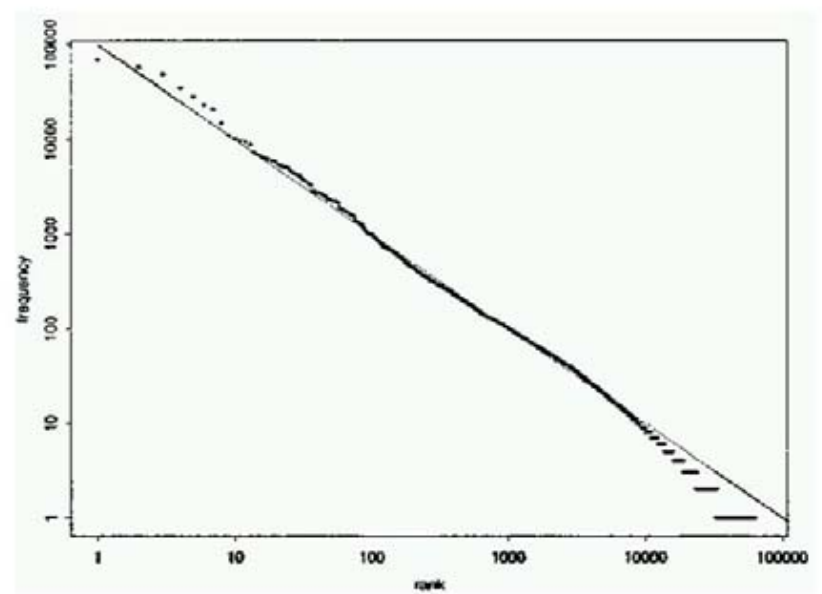
\includegraphics[width=0.8\textwidth]{./images/zipfs_law_brown_corpus.png}
    \caption{Zipf's Law Modelled on the Brown Corpus}
\end{figure}

As can be seen above, Zipf's law is an accurate model excepting the extremes.

\subsection{Vocabulary Growth}
The manner in which the size of the vocabulary increases with the size of the document collection has an impact on our choice of indexing strategy \& algorithms.
However, it is important to note that the size of a vocabulary is not really bounded in the real world due to the existence of mispellings, proper names etc., \& document identifiers.
\\\\
If $V$ is the size of the vocabulary and $n$ is the length of the document collection in word occurrences, then
\begin{align*}
    V = K \cdot n^\beta, \quad 0 < \beta < 1
\end{align*}
where $K$ is a constant scaling factor that determines the initial vocabulary size of a small collection, usually in the range 10 to 100, and $\beta$ is constant controlling the rate at which the vocabulary size increases usually in the range 0.4 to 0.6.

\subsection{Weighting Schemes}
The quality of performance of an IR system depends on the quality of the weighting scheme; we want to assign high weights to those terms with a high resolving power.
tf-idf is one such approach wherein weight is increased for frequently occurring terms but decreased again for those that are frequent across the collection.
The ``bag of words'' model is usually adopted, i.e., that a document can be treated as an unordered collection of words.
The term independence assumption is also usually adopted, i.e., that the occurrence of each word in a document is independent of the occurrence of other words.

\begin{tcolorbox}[colback=gray!10, colframe=black, title=\textbf{``Bag of Words'' / Term Independence Example}]
    If Document 1 contains the text ``Mary is quicker than John'' and Document 2 contains the text ``John is quicker than Mary'', then Document 1 \& Document 2 are viewed as equivalent.
\end{tcolorbox}

However, it is unlikely that 30 occurrences of a term in a document truly carries thirty times the significance of a single occurrence of that term.
A common modification is to use the logarithm of the term frequency:
\begin{align*}
    \text{If } \textit{tf}_{i,d} > 0 \text{:}&   \quad w_{i,d} = 1 + \log(\textit{tf}_{i,d})\\
    \text{Otherwise:}&          \quad w_{i,d} = 0
\end{align*}

\subsubsection{Maximum Term Normalisation}
We often want to normalise term frequencies because we observe higher frequencies in longer documents merely because longer documents tend to repeat the same words more frequently.
Consider a document $d^\prime$ created by concatenating a document $d$ to itself:
$d^\prime$  is no more relevant to any query than document $d$, yet according to the vector space type similarity $\text{sim}(d^\prime, q) \geq \text{sim}(d,q) \, \forall \, q$.
\\\\
The formula for the \textbf{maximum term normalisation} of a term $i$ in a document $d$ is usually of the form
\begin{align*}
\textit{ntf} = a + \left( 1 - a \right) \frac{\textit{tf}_{i,d}}{\textit{tf}\text{max}(d)}
\end{align*}
where $a$ is a smoothing factor which can be used to dampen the impact of the second term.
\\\\
Problems with maximum term normalisation include:
\begin{itemize}
    \item   Stopword removal may have effects on the distribution of terms: this normalisation is unstable and may require tuning per collection.
    \item   There is a possibility of outliers with unusually high frequency.
    \item   Those documents with a more even distribution of term frequencies should be treated differently to those with a skewed distribution.
\end{itemize}

More sophisticated forms of normalisation also exist, which we will explore in the future.

\subsubsection{Modern Weighting Schemes}
Many, if not all of the developed or learned weighting schemes can be represented in the following format
\begin{align*}
    \text{sim}(q,d) = \sum_{t \in q \cap d} \left( \textit{ntf}(D) \times \textit{gw}_t(C) \times \textit{qw}_t(Q) \right)
\end{align*}
where 
\begin{itemize}
    \item   $\textit{ntf}(D)$ is the normalised term frequency in a document.
    \item   $\textit{gw}_t(C)$ is the global weight of a term across a collection.
    \item   $\textit{qw}_t(Q)$ is the query weight of a term in a query $Q$.
\end{itemize}

The \textbf{Okapi BM25} weighting scheme is a standard benchmark weighting scheme with relatively good performance, although it needs to be tuned per collection:
\begin{align*}
    \text{BM25}(Q,D) = \sum_{t \in Q \cap D} \left( \frac{\textit{tf}_{t,D} \cdot \log \left( \frac{N - \textit{df}_t + 0.5}{\textit{df} + 0.5} \right) \cdot \textit{tf}_{t, Q}}{\textit{tf}_{t,D} + k_1 \cdot \left( (1-b) + b \cdot \frac{\textit{dl}}{\textit{dl}_\text{avg}} \right)} \right)
\end{align*}

The \textbf{Pivoted Normalisation} weighting scheme is also as standard benchmark which needs to be tuned for collection, although it has its issues with normalisation:
\begin{align*}
    \text{piv}(Q,D) = \sum_{t \in Q \cap D} \left( \frac{1 + \log \left( 1 + \log \left( \textit{tf}_{t, D} \right) \right)}{(1 - s) + s \cdot \frac{\textit{dl}}{\textit{dl}_\text{avg}}} \right) \times \log \left( \frac{N+1}{\textit{df}_t} \right) \times \textit{tf}_{t, Q}
\end{align*}

The \textbf{Axiomatic Approach} to weighting consists of the following constraints:
\begin{itemize}
    \item   \textbf{Constraint 1:} adding a query term to a document must always increase the score of that document.
    \item   \textbf{Constraint 2:} adding a non-query term to a document must always decrease the score of that document.
    \item   \textbf{Constraint 3:} adding successive occurrences of a term to a document must increase the score of that document less with each successive occurrence.
            Essentially, any term-frequency factor should be sub-linear.
    \item   \textbf{Constraint 4:} using a vector length should be a better normalisation factor for retrieval.
            However, using the vector length will violate one of the existing constraints.
            Therefore, ensuring that the document length factor is used in a sub-linear function will ensure that repeated appearances of non-query terms are weighted less.
\end{itemize}

New weighting schemes that adhere to all these constraints outperform the best known benchmarks.

\section{Relevance Feedback}
We often attempt to improve the performance of an IR system by modifying the user query;
the new modified query is then re-submitted to the system.
Typically, the user examines the returned list of documents and marks those which are relevant.
The new query is usually created via incorporating new terms and re-weighting existing terms.
The feedback from the user is used to re-calculate the term weights.
Analysis of the document set can either be \textbf{local analysis} (on the returned set) or \textbf{global analysis} (on the whole document set).
This feedback allows for the re-formulation of the query, which has the advantage of shielding the user from the task of query reformulation and from the inner details of the comparison algorithm.

\subsection{Feedback in the Vector Space Model}
We assume that relevant documents have similarly weighted term vectors.
$D_r$ is the set of relevant documents returned, $D_n$ is the set of the non-relevant documents returned, and $C_r$ is the set of relevant documents in the entire collection.
If we assume that $C_r$ is known for a query $q$, then the best vector for a query to distinguish relevant documents from non-relevant documents is
\[
    \vec{q} = \left( \frac{1}{\left|C_r\right|} \sum_{d_j \in C_r}d_j \right) - \left( \frac{1}{N - \left|C_r\right|} \sum_{d_j \notin C_r} d_j \right)
\]

However, it is impossible to generate this query as we do not know $C_r$.
We can however estimate $C_r$ as we know $D_r$ which is a subset of $C_r$: the main approach for doing this is the \textbf{Rocchio Algorithm:}
\[
    \overrightarrow{q_{\text{new}}} = \alpha \overrightarrow{q_\text{orginal}} + \frac{\beta}{\left| D_r \right|} \sum_{d_j \in D_r} d_j - \frac{\gamma}{\left| D_n \right|} \sum_{d_j \in D_n}d_j
\]

where $\alpha$, $\beta$, \& $\gamma$ are constants which determine the importance of feedback and the relative importance of positive feedback over negative feedback.
Variants on this algorithm include:
\begin{itemize}
    \item   \textbf{IDE Regular:}
            \[
                \overrightarrow{q_\text{new}} = \alpha \overrightarrow{q_\text{old}} + \beta \sum_{d_j \in D_r} d_j - \gamma \sum_{d_j \in D_n} d_j
            \]

    \item   \textbf{IDE Dec Hi:} (based on the assumption that positive feedback is more useful than negative feedback)
            \[
                \overrightarrow{q_\text{new}} = \alpha \overrightarrow{q_\text{old}} + \beta \sum_{d_j \in D_r} d_j - \gamma \text{MAXNR}(d_j)
            \]
            where $\text{MAXNR}(d_j)$ is the highest ranked non-relevant document.
\end{itemize}

The use of these feedback mechanisms have shown marked improvement in the precision \& recall of IR systems.
Salton indicated in early work on the vector space model that these feedback mechanisms result in an average precision of at least 10\%.
\\\\
The precision-recall is re-calculated for the new returned set, often with respect to the returned document set less the set marked by the user.

\subsection{Pseudo-Feedback / Blind Feedback}
In \textbf{local analysis}, the retrieved documents are examined at query time to determine terms for query expansion.
We typically develop some form of term-term correlation matrix. 
To quantify connection between two terms, we expand the query to include terms correlated to the query terms.

\subsubsection{Association Clusters}
To create an \textbf{association cluster}, first create a matrix $M$;
We can create term $\times$ term matrix to represent the level of association between terms.
This is usually weighted according to
\[
    M_{i,j} = \frac{\text{freq}_{i,j}}{\text{freq}_{i} + \text{freq}_{j} - \text{freq}_{i,j}}
\]

To perform query expansion with local analysis, we can develop an association cluster for each term $t_i$ in the query.
For each term $t_i \in q$ choose the $i^\text{th}$ query term and select the top $N$ values from its row in the term matrix.
For a query $q$, select a cluster for each query term so that $\left| q \right|$ clusters are formed.
$N$ is usually small to prevent generation of very large queries.
We may then either take all terms or just those with the highest summed correlation.

\subsubsection{Metric Clusters}
Association clusters do not take into account the position of terms within documents: \textbf{metric clusters} attempt to overcome this limitation.
Let $\text{dis}(t_i, t_j)$ be the distance between two terms $t_i$ \& $t_j$ in the same document.
If $t_i$ \& $t_j$ are in different documents, then $\text{dis}(t_i, t_j) = \inf$.
We can define the term-term correlation matrix by the following equation, and we can define clusters as before:
\[
    M_{i,j} = \sum_{t_i, t_j \in D_i} \frac{1}{\text{dis}(t_i, t_j)}
\]

\subsubsection{Scalar Clusters}
\textbf{Scalar clusters} are based on comparing sets of words:
if two terms have similar neighbourhoods then there is a high correlation between terms.
Similarity can be based on comparing the two vectors representing the neighbourhoods.
This measure can be used to define term-term correlation matrices and the procedure can continue as before.

\subsection{Global Analysis}
\textbf{Global analysis} is based on analysis of the whole document collection and not just the returned set.
A similarity matrix is created with a similar technique to the method used in the vector space comparison.
We then index each term by the documents in which the term is contained.
It is then possible to calculate the similarity between two terms by taking some measure of the two vectors, e.g. the dot product.
To use this to expand a query, we then:
\begin{enumerate}
    \item   Map the query to the document-term space.
    \item   Calculate the similarity between the query vector and vectors associated with query terms.
    \item   Rank the vectors $\vec{t_i}$ based on similarity.
    \item   Choose the top-ranked terms to add to the query.
\end{enumerate}

\subsection{Issues with Feedback}
The Rocchio \& IDE methods can be used in all vector-based approaches.
Feedback is an implicit component of many other IR models (e.g., neural networks \& probabilistic models).
The same approaches with some modifications are used in information filtering.
Problems that exist in obtaining user feedback include:
\begin{itemize}
    \item   Users tend not to give a high degree of feedback.
    \item   Users are typically inconsistent with their feedback.
    \item   Explicit user feedback does not have to be strictly binary, we can allow a range of values.
    \item   Implicit feedback can also be used, we can make assumptions that a user found an article useful if:
            \begin{itemize}
                \item   The user reads the article.
                \item   The user spends a certain amount of time reading the article.
                \item   The user saves or prints the article.
            \end{itemize}

            However, these metrics are rarely as trustworthy as explicit feedback.
\end{itemize}



\end{document}
